%=============================================================================
% THIS IS .....    chapter{EID: The Error Insertion Device } ........
% Revisions
% Nov.95 - Simao Campos
% Jan.96 - Peter Kroon, Simao Campos, Paul Voros, Rosario D. de Iacovo,
% Mar.96 - Simao Campos
% Apr.96 - Peter Kroon
% Feb.2000 - Convergence towards STL2000
% Oct.2009 - EID-EV Jonas Svedberg, Yusuke Hiwasaki
%=============================================================================

%=============================================================================
\chapter{EID: Error Insertion Device}
%=============================================================================

An error insertion device (EID) is used to study the behaviour of
codec over digital transmission systems and equipments under error
conditions. This requires a model for the transmission channel, and an
error generation algorithm. In the most general case, burst or random
bit error generators are needed. In other cases, such as when
evaluating mobile and wireless systems, random and bursty frame
erasures are of importance.

The EID module implements the four functionalities: random and bursty
bit errors, and random and bursty frame erasures. These four models
are based on a linear congruential sequence random number generator,
and the bit error insertion and random frame erasure are based on a
two-state channel model.

The burst frame erasure function requires a more elaborated model. For
the specific application of wireless systems, a model based on Markov
sequences is used. This is known within ITU as the Bellcore model
\cite{Bellcore-Model-1,Bellcore-Model-2}. This model was first used in
the standardization of ITU-T G.729, and has been incorporated in the
STL since.

Upon development needs of scalable and embedded-variable bitrate
codecs, a more elaborate EID simulation software was added in STL2009
release. This tools allows more complex error insertion simulations:
layered application mode where upper layers are dependent on the error
of lower layers, and (optional) individual application mode where
errors are inserted separately to each layer. 

%--------------------------------------
\section{Description of Algorithm}
%--------------------------------------

%................................
\subsection{Simple Channel Model}

The bit error insertion algorithm of the EID is based on a channel model
where (binary) data bitstreams are to be transmitted, and is based on the
discrete {\it Gilbert Elliott channel} (GEC) model, described in
\cite{GEC}.

This model (see figure \ref{GEC}) has two states, Good ($G$) and
Bad or Burst ($B$). Associated with these two states, there are four
parameters (probabilities): two relating to the probability of remaining
in state $G$ or $B$, and two relating to the probability of transition from
the current state to the other state (i.e., the occurrence of a
binary digit transition, or error).

The probabilities associated with the channel states are $P$ and $Q$, $P$
being the probability of transition from state $G$ to $B$, and $Q$ the
probability of transition from $B$ to $G$. Hence, the probability of
remaining in the same state is $(1-P)$ and $(1-Q)$ for states $G$ and $B$,
respectively. For a given state, there are probabilities that a change in
a bit occur, and this is $P_G$ for state $G$, and $P_B$ for state $B$.

Therefore, the channel may be either in the good state $G$, where the
mean bit error probability $P_G$ is very low ($P_G \approx 0$), or in
the bad state $B$, where the mean bit error probability $P_B$ is rather
high ($P_B \approx 0.5$). \\

\begin{figure}[hb]
    \begin{center}
%        \includegraphics{GilbertElliotChannelModel.ps}
        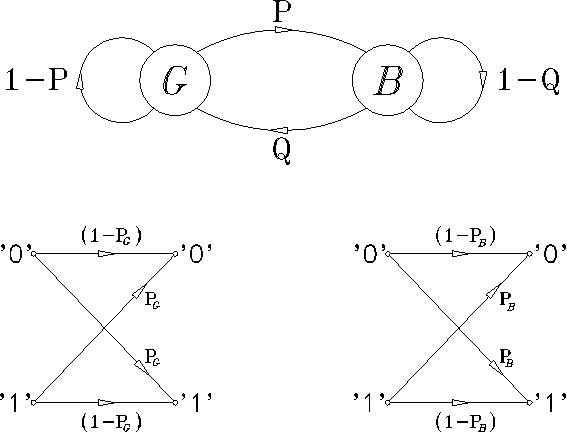
\includegraphics{GilbertElliotChannelModel}
    \end{center}
    \caption{{\label{GEC}} Gilbert Elliot Channel Model (GEC)}
\end{figure}

The mean bit error probability {\em BER} generated by this channel model is
\begin{equation} \label{EQ1}
                 \BER \ \ =\ \ \frac{P}{1-\gamma}\cdot P_B \ \
                          +\ \ \frac{Q}{1-\gamma}\cdot P_G
\end{equation}
where
\begin{equation} \label{EQ2}
                           \gamma \ \ =\ \ 1-(P+Q)
\end{equation}

is a measure for the correlation of the bit errors, and consequently an
indication of the burst or random characteristic of the channel. In
this issue, $\gamma \approx 0$ implies a nearly random error channel,
while $\gamma \approx 1$ implies a totally bursty channel. Please note
that {\em BER} is reasonable only in the range $0 \le \BER \le 0.5$.\\

For many applications, bit error sequences with a distinct mean bit
error probability {\em BER} and a distinct bit error correlation
$\gamma$ are of interest. From equations (\ref{EQ1}) and (\ref{EQ2}) we
get for the remaining parameters of the $GEC$ for arbitrarily chosen
values of $0 \le P_G < P_B \le 0.5$:

\begin{eqnarray} \label{EQ3}
        P & = & (1-\gamma) \ \ \cdot \ \ (1-\frac{P_B-\BER}{P_B-P_G})\\
                                &&\nonumber \\
        Q & = & (1-\gamma) \ \ \cdot \ \ \frac{P_B-\BER}{P_B-P_G} \label{EQ4}
\end{eqnarray}

In the Error Insertion Device (EID) the special values $P_G=0$ and
$P_B=0.5$ are chosen. This relates to the fact that in the good state
no bit changes are expected, hence $P_G=0$; now, for the bad state, the
channel is supposed to be in a totally uncertain state, then $P_B=0.5$.
With this choice, equations (\ref{EQ3}) and (\ref{EQ4}) reduce to:

\begin{eqnarray} \label{EQ5}
                   P & = & 2 \cdot (1-\gamma) \cdot \BER \\
                                && \nonumber\\
                   Q & = & (1-\gamma) \cdot (1-2 \cdot \BER) \label{EQ6}
\end{eqnarray} \ \\

As an example, figure \ref{Gamma} shows the effect of $\gamma$ on the
auto-correlation of a bitstream, generated by the $GEC$ (with $\BER = 0.02$
in equations (\ref{EQ5}),(\ref{EQ6})).

%----------------------------------------------------------------------
% Correlation function plot
%----------------------------------------------------------------------
\begin{figure}[hb]
    \begin{center}
%        \includegraphics{BitErrorCorrelation.ps}
        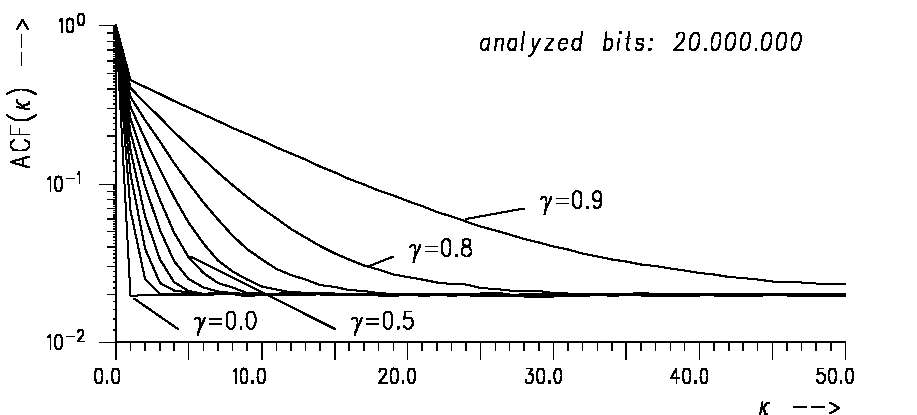
\includegraphics{BitErrorCorrelation}
    \end{center}
    \caption{{\label{Gamma}} Bit Error
                Correlation for a Bit Error Rate of 2\%}
\end{figure}
%----------------------------------------------------------------------

It can be seen that for $\gamma=0$ the bit errors are statistically
independent, because the autocorrelation sequence ACF$(\kappa)$ has a peak
(1.0) in $\kappa=0$, and the remaining coefficients ACF(1),ACF(2),... oscillate
around the selected bit error rate of 0.02 ($2 \cdot 10^{-2}$). For
$\gamma=0.5$, slightly bursty errors can be observed, when the initial terms
of the correlation sequence build a transition region, and the remaining
(higher) terms are around 0.02. Increasing $\gamma$ towards unity, the
correlation between the bit errors also increases, leading to totally bursty
errors in the limit.\\

%................................
\subsection{Bellcore Model}

The following description has been based on \cite{Bellcore-Model-1}. The
actual error sequence in a wireless environment will depend upon the
carrier frequency, user speed, detection scheme, type of diversity
employed, mean SNR, hand-off mechanism, etc. Though a model could be
created using the above parameters, it would be impossible to apply
because of the wide variance of the model parameters. It was found that a
speech coder can be tested using error bursts generated by a much simpler
model because the burst error performance of a speech coder can be
characterized to a great extend by the way it reacts to short (5--20 ms),
medium (30--60 ms) and long (over 80 ms) error bursts. If a coder performs
well in the presence of a representative range of short, medium and long
error bursts, it can be expected that the coder will behave well in an
actual wireless communications environment, even though the actual radio
channel generates error bursts with different statistics.

The Bellcore model, rather than modeling the wireless communications channel,
models the occurrence of these short, medium, and long error bursts that would
enable the characterization of the coder reaction
to error bursts and to the error burst patterns it is expected it will
encounter in practice.

%----------------------------------------------------------------------
% N-state Markov model
%----------------------------------------------------------------------
\begin{figure}[hb]
  \begin{center}
    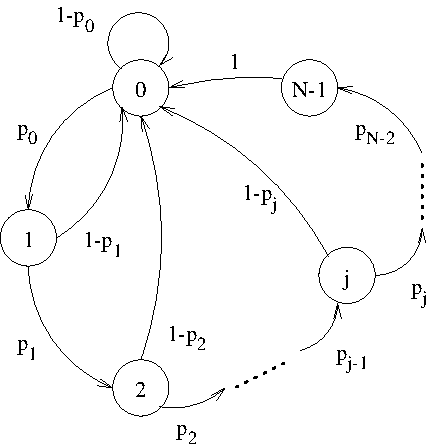
\includegraphics{nsmarkov}
  \end{center}
  \caption{\label{N-state-Markov} N-state Markov Model.}
\end{figure}
%----------------------------------------------------------------------

An N-state Markov model, as illustrated in figure \ref{N-state-Markov}, is
used in the STL to generate frame erasure bursts. This model has to be
adequate to test speech coders using short speech segments (6-8s). In this
model, a transition from any state (0..N--1) to state 0 represents a frame
received without errors, while a transition from state j--1 to state j
indicates that j previous frames have been received in error. A transition
from j back to 0 marks the end of an error burst of length j followed by a
good frame.

The Markov model with N states for creating a bursty wireless communications
channel is capable of erasing up to N--1 frames. The model generates both
frames with correlated frame erasures and error-free frames. The value of N
will depend on the frame duration of the speech coder under test and the
maximum error burst length the coder expects to find in practice. The error
statistics can be controlled by selecting the N--1 transition probabilities
$p_k$, $k$=0..N--2. The probabilities will also determine the sequence of
good and erased frames.

The steady state probabilities can be calculated by solving the state
transition matrix or using numerical methods. If $S_j$
denotes the steady state probability that the chain is in state
$j$ and $p_j$ is the probability of transitioning from state $j$ to $j+1$,
the following relationships can be established:
\[
    S_{j+1} = p_j S_j \mbox{\rule{20mm}{0mm}} 0 \le j \le N-2
\]

\[
   S_0 = \sum_{j=0}^{N-1} S_j (1-p_j) \mbox{\rule{15mm}{0mm}} (p_{N-1}=0)
\]

The equations above can be solved since the probabilities should satisfy:
\[
   \sum_{j=0}^{N-1} p_j = 1
\]

A frame erasure length of $j$ can occur only if the chain first enters state
$j$, and then transitions to state 0. The probability $P_{fe}$ of this
occur is
\[
   P_{fe} = S_j (1-p_j)
\]

The probability of receiving a frame in error can be calculated as
\[
   P_e = \sum_{j=1}^{N-1} j P_{fe}(j)
\]
and the probability of receiving an error-free frame is $1-P_e$. It
can be seen that the steady state probability of being in state 0, $S_0$,
also gives the probability of receiving a frame without error, i.e.,
\[
  S_0 = 1 - \sum_{j=1}^{N-1} j P_{fe}(j)
\]

The frame error distribution can be controlled by selecting the transition
probabilities.

%\textcolor{red}{
%--------------------------------------
\subsection{Error insertion for layered bitstreams}
%--------------------------------------
%}

A layered scalable codec provides a multi-layer bitstream that can be 
modified by application or network entities:
\begin{itemize}
\item The core layer of the codec provides a minimum quality. 
\item Upper layers enable improving quality by increasing bitrate up
  to a maximum value.
\end{itemize}
One main feature of a scalable codec lies in the layering flexibility. 
The layers can be transported over different channels or over the same 
channel but with different priorities. Further the bitrate can be adjusted 
between minimal and maximal values by any network element in the 
communication chain. 

To simulate the layering functionality a bitstream error application
tool (eid-ev) was added for STL2009 release. This tool applies layer
errors at desired levels. For each frame of an input bitstream, this
tool performs the following operations:
\begin{enumerate}
\item Read and validate the input frame, (each input frame size needs
  to represent a valid layer boundary) 
\item	Read the frame error pattern files, (one error pattern file is
  read for each layer)
\item Apply errors by copying non-distorted layers to the output
  frame, and setting the bits of distorted layers to the softbit value
  zero. 
\item Truncate output frame if consecutive higher layers are hit by errors.
\item Set the correct synchronization header of the output frame
\item Set the correct length of the output frame.
\item Provide statistics of error application across layers.
\end{enumerate}

%--------------------------------------
\section{Implementation}
%--------------------------------------

The EID algorithm is written in C-source code can be found in the
module {\tt eid.c}, with prototypes in {\tt eid.h}. This version
evolved from previous C implementations developed by PKI\footnote{\SF
  Phillips Communications Industry.}, and was used in the Host
Laboratory Sessions of ETSI's contest for the second generation of the
GSM Digital Mobile Radio Systems, and in the Selection Phase of the
ITU-T 8 kbit/s speech coder.

The random-number generator is based on a linear congruential
technique, as described in \cite{Knuth}. The rule here is:
\[
   a_n = (69069 * a_{n-1} +1 ) \bmod 2^{32}\mbox{,}
\]
which is converted (mapped) to a float number between 0 and 1.

Since the random number generator and the channel need their internal
state to be saved, two state variable data structure types were defined
for the EID module. The structure type called {\tt SCD\_EID} is applicable
to the burst and random bit erasure functions, as well as to the random
frame erasure function. The fields of this structure are:
\begin{quote} \normalsize
 {\em seed}     \hfill \pbox{110mm}{\SF Seed for random number
                                          generator. }\\*[1mm]
 {\em nstates}  \hfill \pbox{110mm}{\SF Number of states of the
                                          channel model (presently 2).}\\*[1mm]
 {\em current\_state} \hfill \pbox{110mm}{\SF Index of current
                                          channel state. }\\*[1mm]
 {\em ber}      \hfill \pbox{110mm}{\SF Pointer to array containing
                                          thresholds according to the
                                          bit error rate in each state.
                                         }\\*[2mm]
 {\em usrber}   \hfill \pbox{110mm}{\SF User defined bit error rate. }\\*[1mm]
 {\em usrgamma} \hfill \pbox{110mm}{\SF User defined correlation
                                          factor. }\\*[1mm]
 {\em matrix}   \hfill \pbox{110mm}{\SF Pointer to matrix containing
                                          thresholds according to the
                                          probabilities for changing from one
                                          state to another one. }\\
\end{quote}

For burst frame erasures only, a different state variable structure type
called {\tt BURST\_EID} has been defined, whose fields are:
\begin{quote} \normalsize
 {\em seedptr}     \hfill \pbox{110mm}{\SF Memory for random
                                          number generator. }\\*[1mm]
 {\em internal}  \hfill \pbox{110mm}{\SF Array with
                                          probabilities for each state of
                                          the Markov process.}\\*[1mm]
 {\em index} \hfill \pbox{110mm}{\SF Channel's current state. }\\
\end{quote}

The values of the fields shall not be altered and are not needed by user.

The random number generator always starts from the same point, if the user
does not specify different initial seeds. In order to avoid this, the
EID state variables should be saved at the end of the processing of a
speech sequence, e.g. to a file by the user. This saving is not
implemented by the EID module because this involves I/O to the computer
file systems, and this would violate one of the UGST guidelines. Nevertheless,
an example of this procedure is described in the demonstration programs that
accompany this release of the EID. Therefore, users should keep in
mind that, unless they save (e.g. to a file) the EID state at the end of
the processing, identical error patterns will be produced, when the
processing is re-started.

The EID routines for random bit errors are {\tt BER\_generator} and
{\tt BER\_insertion}; for random frame erasures, {\tt
FER\_generator\_random} and {\tt FER\_module}; for burst frame
erasures\\ {\tt FER\_generator\_burst}; and {\tt open\_eid}, {\tt
open\_burst\_eid} and {\tt close\_eid} for initialization (allocation)
and release of EID state structures {\tt SCD\_EID} and {\tt
BURST\_EID}. Their description can be found next. Besides these, there
are other routines which are local (private) to the EID module, and
therefore are not described.

%--------------------------------------
\subsection{Bitstream format}\label{sec:g192bitstream}
%--------------------------------------

The EID module operates on {\em softbits} basis. Softbits are defined
as a multi-level representation of the binary (``hard'') bits `1' and
`0' which are associated to probabilities of being in error. The
softbit definition adopted in the ITU-T STL uses 16-bit words as
representation of the hardbits {\tt `1'} and {\tt `0'}, where a
hardbit {\tt `1'} is represented by the softbit {\tt 0x0081} and a
hardbit {\tt `0'} is represented by the softbit {\tt 0x007F}. This
means that 8 significant bits in a softbit is available for other
utilities. When soft-decision is not used, the hard bit information
can be derived directly from Bit~7 of the 16-bit softbit word. It
should also be noted that values {\tt 0x0081} and {\tt 0x007f} are
equally spaced from {\tt 0x0000} (in other words, {\tt 0x0000} is
exactly the middle of the two-complement range for {\tt 0x81} and {\tt
  0x7F}), such that a softbit representation {\tt 0x0000} represents
{\em total uncertainty} of the true bit value.

Error patterns produced and used by the EID module use this softbit
definition. Input and output data (i.e. signals which are affected by
bit errors or frame erasures) also use softbits, but additionally have
a so-called synchronization header.

The {\em synchronization header} is defined as two consecutive 16-bit
words, the first one always being a synchronization (sync) word in the
range {\tt 0x6B21} to {\tt 0x6B2F}, followed by the bitstream length
word, a two-complement number indicating the number of softbits in the
frame. The sync word {\tt 0x6B20} is reserved to indicate that a frame
erasure happened. For example, for the RPE-LTP algorithm, which uses
260 bits per frame, the soft bitstream would have the format indicated
in figure \ref{fig:bs-rpeltp}. It can be seen that each RPE-LTP frame
will have 262 16-bit words, being one for the sync word ({\tt 0x6B21}
in the example), one for the frame length word (whose value here is
260), followed by 260 softbit words (here corresponding to {\tt `1'},
{\tt `0'}, ..., {\tt `0'}, {\tt`0'}). This combination of the
synchronization header and a softbit ``payload'' is called the
bitstream signal representation and is used in ITU-T Recommendation
G.192 \cite{G.192} to represent encoded signals between speech
encoders, error-insertion devices, transmission channel models and
speech decoders.

%----------------------------------------------------------------------
% Example of bitstream format signal
%  Figure created with designer, exported as EPS, no preview, edited to
%  remove trash from its header before usage by LaTeX
%----------------------------------------------------------------------
\begin{figure}[ht]
\begin{center}
    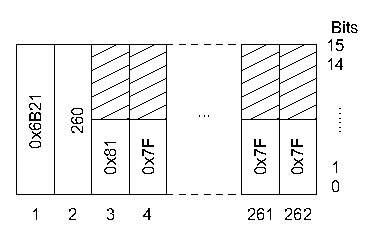
\includegraphics{bsrpeltp}
\end{center}
  \Caption{10cm}{Soft bitstream format for the 13 kbit/s RPE-LTP
           algorithm, where 260 bits are transmitted per 20 ms
           transmission frame.
           \label{fig:bs-rpeltp} }
\end{figure}
%----------------------------------------------------------------------

%.................................
\subsection{{\tt open\_eid}}

{\bf Syntax: }

{\tt
\#include "eid.h"\\
SCD\_EID *open\_eid (\ttpbox{110mm}{
            double {\em ber}, double {\em gamma});
         }
}

{\bf Prototype: }    eid.h

{\bf Description: }

Allocate memory for EID struct, set up the transmission matrix
according to the selected bit error rate, and initialize the seed for
the random number generator. If the symbol {\tt PORT\_TEST} is defined
at compilation time, then the seed will always be initialized to the
same value; otherwise, the seed is initialized with the system time
(in seconds). The former is used to test portability of the EID
module, since identical patterns will be generated\footnote{\SF
Another way to force the EID to produce identical bit error patterns
is to save the EID state variable (of type {\tt SCD\_EID}) e.g. to a
file and, in the next call to the routine, initialize the state
variable with the saved value.}.

{\bf Variables: }
\begin{Descr}{\DescrLen}
\item[\pbox{20mm}{\em ber}] %%\rulex{1mm}\\
        User desired bit error rate;

\item[\pbox{20mm}{\em gamma}] %%\rulex{1mm}\\
        User desired burst factor;
\end{Descr}


{\bf Return value: }

Returns a pointer to struct {\tt SCD\_EID}; if the initialization failed,
returns a null pointer.



\subsection{{\tt open\_burst\_eid}}

{\bf Syntax: }

{\tt
\#include "eid.h"\\
BURST\_EID *open\_burst\_eid (\ttpbox{110mm}{
            long {\em index});
         }
}

{\bf Prototype: }    eid.h

{\bf Description: }

Allocate memory for a state variable structure of type {\tt
BURST\_EID} and setup the transmission matrix according the burst
frame erasure rate (BFER) selected by {\em index}, and initialize the
seed for the random number generator. If the symbol {\tt PORT\_TEST}
is defined at compilation time, then the seed will always be
initialized to the same value; otherwise, the seed is initialized with
the system time, in seconds (see note in the description of {\tt
open\_eid()}).

{\bf Variables: }
\begin{Descr}{\DescrLen}
\item[\pbox{20mm}{\em index}] %%\rulex{1mm}\\

        Indicates BFER index starting from 0\% to 30\% with 0.5\%
        steps for the Bellcore model. If {\em index} is equal to 0,
        there is no FER, and 1 means that there is 0.5\% BFER;
        incrementally, 60 gives 30\% BFER.\\
\end{Descr}


{\bf Return value: }

This function returns a pointer to a structure of type {\tt
BURST\_EID}. If the initialization failed, it returns a null pointer.


%.................................
\subsection{{\tt reset\_burst\_eid}}

{\bf Syntax: }

{\tt
\#include "eid.h"\\
void reset\_burst\_eid (\ttpbox{110mm}{
            BURST\_EID {\em *burst\_eid});
         }
}

{\bf Prototype: }    eid.h

{\bf Description: }

Reset a {\tt BURST\_EID} structure previously initialized by a call to
{\tt open\_burst\_eid()}. By default, only counters are reset; if the
symbol {\tt RESET\_SEED\_AS\_WELL} is defined at compilation time, the
seed is also reset. However, this is not recommended.

{\bf Variables: }
\begin{Descr}{\DescrLen}
\item[\pbox{20mm}{\em burst\_eid}] %%\rulex{1mm}\\
        {\tt BURST\_EID} structure to be reset.
\end{Descr}

{\bf Return value: }

        None.


%.................................
\subsection{{\tt close\_eid}}

{\bf Syntax: }

{\tt
\#include "eid.h"\\
void close\_eid (\ttpbox{110mm}{
            SCD\_EID {\em *EID});
         }
}

{\bf Prototype: }    eid.h

{\bf Description: }

Release the memory previously allocated by {\tt open\_eid()} for the
specified EID structure.

{\bf Variables: }
\begin{Descr}{\DescrLen}
\item[\pbox{20mm}{\em EID}] %%\rulex{1mm}\\
        EID state variables' structure to be released.
\end{Descr}

{\bf Return value: }

        None.

%.................................
\subsection{{\tt BER\_generator}}

{\bf Syntax: }

{\tt
\#include "eid.h"\\
double BER\_generator (\ttpbox{110mm}{
             SCD\_EID {\em *EID}, long {\em lseg}, short {\em *EPbuff});
         }
}

{\bf Prototype: }    eid.h

{\bf Description: }

Generates a softbit error pattern according to the selected channel
model present in {\em EID}. The introduction of the bit errors in the
bitstream is done by the function {\tt BER\_insertion}. It should be
noted that softbit error pattern buffers do not contain
synchronization headers.

{\bf Variables: }
\begin{Descr}{\DescrLen}
\item[\pbox{20mm}{\em EID}] %%\rulex{1mm}\\
         Structure with channel model.

\item[\pbox{20mm}{\em lseg}] %%\rulex{1mm}\\
         Length of current frame.

\item[\pbox{20mm}{\em EPbuff}] %%\rulex{1mm}\\
         Bit error pattern buffer with softbits.
\end{Descr}


{\bf Return value: }

The bit error rate in the current frame is returned as a \double.


%.................................
\subsection{{\tt FER\_generator\_random}}

{\bf Syntax: }

{\tt
\#include "eid.h"\\
double FER\_generator\_random (SCD\_EID {\em *EID});
}

{\bf Prototype: }    eid.h

{\bf Description: }

Decides whether a random frame erasure should happen for the current frame
according to the state of the GEC model in the channel memory
pointed by {\em EID}.

{\bf Variables: }
\begin{Descr}{\DescrLen}
 \item[\pbox{20mm}{\em EID}] Structure with channel model.
\end{Descr}

{\bf Return value: }

Returns a {\tt double} value: 0 if the current frame should not be
erased (``good frame'') and 1 if the frame should be erased (``bad
frame'').


%.................................
\subsection{{\tt FER\_generator\_burst}}

{\bf Syntax: }

{\tt
\#include "eid.h"\\
double FER\_generator\_burst (BURST\_EID {\em *EID}); }

{\bf Prototype: }    eid.h

{\bf Description: }

Decides whether a burst frame erasure should happen for the current
frame according to the state of the Bellcore model in the channel
memory pointed by {\em EID}. It should be noted that in the long run,
the overall burst frame erasure rate (BFER) may not be consistent with
the BFER specified by the user. This is an inherent deficiency of the
implemented model and the calling program is responsible for computing
the overall BFER and monitoring whether this overall BFER is close
enough to the desired BFER.

{\bf Variables: }
\begin{Descr}{\DescrLen}
 \item[\pbox{20mm}{\em EID}] Structure with Bellcore model parameters.
\end{Descr}

{\bf Return value: }

This function returns a {\tt double} value: 0 if the current frame
should not be erased (``good frame'') and 1 if the frame should be
erased (``bad frame'').

%.................................
\subsection{{\tt BER\_insertion}}

{\bf Syntax: }

{\tt
\#include "eid.h"\\
void BER\_insertion (\ttpbox{110mm}{
             long {\em lseg}, short {\em *xbuff}, short {\em *ybuff},
             short {\em *error\_pattern});
         }
}

{\bf Prototype: }    eid.h

{\bf Description: }

Disturbs an input bitstream {\em xbuff} according to the error pattern
provided in {\em error\_pattern}, saving the disturbed bitstream in
the output buffer {\em ybuff}. The input and output bitstream are
compliant to the bitstream format described before, i.e. are comprised
of a synchronization header (sync word followed by a frame length
word) and softbits representing the encoded bitstream. The sync and
frame length words are always located in the offsets 0 and 1 of the
array, respectively. The error pattern contains only softbits. The
following summarizes the bit error insertion rules:

\def\labelenumi{\alph{enumi})}
\def\theenumi{\alph{enumi}}

\begin{enumerate}
 \item input signal (after synchronization header):

     $\bullet$ hard bit {\tt '0'} represented as {\tt 0x007F}; \\
     $\bullet$ hard bit {\tt '1'} represented as {\tt 0x0081}.\\

 \item error pattern:

       $\bullet$ the probability for undisturbed transmission has values
                 in the range {\tt 0x0001..\-0x007F}, \rulex{3em}
                 being {\tt 0x0001} the lowest probability.

       $\bullet$ the probability for disturbed transmission has values
                 in the range {\tt 0x00FF..\-0x0081}, \rulex{3em}
                 being {\tt 0x00FF} the lowest probability.

 \item output signal computation (does not affect the synchronization
        header, which is copied unmodified from the input buffer to
        the output buffer):

        For input {\tt `1'} ({\tt 0x0081}): \\
         \rulex{5mm} $\bullet$ \pbox{120mm}{
                if the error pattern is in the range {\tt 0x00FF..0x0081}
                (255..129), then the output will be {\tt 0x0001..0x007F}
                (1..127), respectively;}

         \rulex{5mm} $\bullet$ \pbox{120mm}{
                if the error pattern is in the range {\tt 0x0001..0x007F}
                (1..127), then the output will be {\tt 0x00FF..0x0081}
                (255..129), respectively.}

        For input {\tt `0'} ({\tt 0x007F}): \\
         \rulex{5mm} $\bullet$ \pbox{120mm}{
                if the error pattern is in the range {\tt 0x00FF..0x0081}
                (255..129), then the output will be {\tt 0x00FF..0x0081}
                (255..129), respectively;}

         \rulex{5mm} $\bullet$ \pbox{120mm}{
                if the error pattern is in the range {\tt 0x0001..0x007F}
                (1..127), then the output will be {\tt 0x0001..0x007F}
                (1..127), respectively.}
\end{enumerate}

\def\labelenumi{\arabic{enumi}.}
\def\theenumi{\arabic{enumi}}


{\bf Variables: }
\begin{Descr}{40mm}
\item[\pbox{20mm}{\em lseg}] %%\rulex{1mm}\\
            Length of current frame (including synchronization
            header). \smallskip

\item[\pbox{20mm}{\em xbuff}] %%\rulex{1mm}\\
            Buffer with input bitstream of length {\em lseg}.\smallskip

\item[\pbox{20mm}{\em ybuff}] %%\rulex{1mm}\\
            Buffer with output bitstream of length {\em lseg}.\smallskip

\item[\pbox{25mm}{\em error\_pattern}] %%\rulex{1mm}\\
            Buffer with error pattern (without synchronization header),
            of length {\em lseg--2}.
\end{Descr}

{\bf Return value: }

        None.

%.................................
\subsection{{\tt FER\_module}}

{\bf Syntax: }

{\tt
\#include "eid.h"\\
double FER\_module (\ttpbox{110mm}{
             SCD\_EID {\em *EID}, long {\em lseg}, short {\em *xbuff},
             short {\em *ybuff});
         }
}

{\bf Prototype: }    eid.h

{\bf Description: }

Implementation of the frame erasure function based on the GEC model
allowing a variable degree of burstiness (as specified by parameter
{\tt gamma} in the state variable structure of type {\tt SCD\_EID}
pointed by {\em EID}). This function actually erases the current frame (as
described below), as opposed to function {\tt
FER\_generator\_random()}, which only indicates whether the current
frame should be erased.

\rulex{5mm} \begin{minipage}{150mm}
        $\bullet$ computes the ``frame erasure pattern'';

        $\bullet$ erases all bits in one frame according the current
          state of the pattern generator.
\end{minipage}

The input (undisturbed) and output (disturbed) buffers have samples
conforming to the bitstream representation description in Annex B of
G.192. The input and output bitstream are compliant to the bitstream
format described before, i.e. are comprised of a synchronization
header (sync word followed by a frame length word) and softbits
representing the encoded bitstream. The sync and frame length words
are always located in the offsets 0 and 1 of the array,
respectively. Should the frame be erased (depending on the frame
erasure pattern), all softbits are set to {\tt 0x0000}, which
corresponds to a total uncertainty about the true bit values.

In addition, the lower 4 bits of the sync word in the synchronization
header are set to 0. This makes it easier for the succeeding software
to detect an erased frame. The frame length word is copied unmodified
to the output buffer.


{\bf Variables: }
\begin{Descr}{\DescrLen}
\item[\pbox{20mm}{\em EID}] %%\rulex{1mm}\\
        Pointer to a state variable structure structure of type {\tt SCD\_EID}.

\item[\pbox{20mm}{\em lseg}] %%\rulex{1mm}\\
        Length of current frame (including synchronisation header).

\item[\pbox{20mm}{\em xbuff}] %%\rulex{1mm}\\
        Pointer to input bitstream. The synchronisation word ({\em xbuff[0]})
        is processed, the frame length word ({\em xbuff[1]}) is not changed.

\item[\pbox{20mm}{\em ybuff}] %%\rulex{1mm}\\
        Buffer with output bitstream.
\end{Descr}


{\bf Return value: }

This function returns a {\tt double} value: 1 if the current frame has
been erased, and 0 otherwise.

%--------------------------------------
\section {Tests and portability} \label{EID-Tests}
%--------------------------------------

Portability may be checked by running the same speech file on a proven
platform and on a test platform, for the whole range of input
parameters. Results should be identical when the compilation is done
with the symbol {\tt PORT\_TEST} properly defined and the channel
states are set to a same value.

For the eid-ev program, please note that the 16 bit oriented G.192 files 
require correct byte swapping of inputs and outputs on big/little-endian 
machines. It checks for inconsistent sync headers and exits the program with 
a warning if incorrectly swapped synchronism headers are detected. 

The original EID routines had portability tested for VAX/VMS with
VAX-C, MS-DOS with Turbo C v2.0, Sun-OS with Sun-C, and HPUX with
gcc. The newly introduced eid-ev programs were tested for Microsoft
C-compiler and gcc on Cygwin.


%--------------------------------------
\section {Examples}
%--------------------------------------

%..........................................................................
\subsection {Description of demonstration programs}

Number of programs are provided as demonstration programs for the EID
module, eiddemo.c (version 3.2), eid8k.c (version 3.2), eid-xor.c
(version 1.0), gen-patt.c (version 1.4), ep-stats.c (version 2.0),
eid-int.c (version 1.0), eid-ev.c (version 1.0), gen\_rate\_profile.c
(version 1.2).

Program {\tt eiddemo.c} uses input and output file in the form of a
serial bit stream conforming to the bitstream signal representation,
as defined in Annex B of ITU-T G.192. This program will disturb the
input bitstream with errors using the Gilbert Elliot Channel model for
random or burst bit error insertion and for random frame erasures. The
Bellcore model, which is used for burst frame erasures, is supported
as a command line option, but not as default. It should be noted that
this program uses function {\tt FER\_module()}, not function {\tt
FER\_generator\_random()}, for random frame erasures.

Program {\tt eid8k.c} was developed during the standardization process of
the ITU-T G.729 8 kbit/s speech codec for the task of producing bit
error masks which would be used in the host laboratory
hardware-implemented EID. For this program, input files are not
generated, but only bit error pattern files. Consistent with the
definition in the STL, error patterns do not have synchronization
headers (sync word and frame length word), but only softbits
representing disturbance of the channel. GEC and the Bellcore model
are supported in this program. The output file format is, as was
necessary for the G.729 work, different from a serial bitstream as
defined in the STL because the softbits are saved as {\tt char} (8-bit
words) rather than as {\tt short} (16-bit words). Conversion of this format
to the STL 16-bit bitstream format can be accomplished using the
unsupported program {\tt ch2sh.c}.

It should be noted that both programs save in files the current
state of the EID models under use and also try to read
these state files at startup time (if not found, the programs create
new ones, which are updated when the programs terminate).

Program {\tt eid-xor.c} is an error-insertion program that simply XORs
bits in a bitstream file (in one out of three formats: G.192,
byte-oriented G.192, and compact) with error patterns (bit errors or
frame erasures in one out of three formats) and saves the disturbed
bitstream in a file. The error patterns need not have been produced by
any of the EID models implemented in the STL, they only have to be in
one of the three input formats. Since error patterns are either bit
error EPs or frame erasure EPs, simultaneous bit errors and frame
erasures are not allowed by {\tt eid-xor.c}.

The program {\tt gen-patt.c} is used to generate error patterns (EPs) using
the EID models implemented in the STL (Gilbert and Bellcore
models). The EPs will be either frame erasures or bit errors EPs,
since the models in the STL do not support mixed frame erasure/bit
error mode.

Program {\tt ep-stats.c} examines an error pattern file (either bit
error EPs or frame erasure EPs) and displays the actual BER/FER found
in the EP and the distribution of number of consecutive errored bits
or erased frames.

Program {\tt eid-int.c} interpolates a frame erasure EP such that each
synchronism word found in the EP is repeated a user-specified number
of times. This is useful to align the frame erasures for codecs that
have frame sizes that are an integer sub-multiple of each other
(e.g. 10ms codecs and 20 ms codecs). In the latter example, the master
EP will be the 20ms one, and the one generated by eid-int would be
used for the 10ms codec.

Program {\tt eid-ev.c} performs an error insertion for layered G.192
files.  This program can be used to apply errors to individual layers
in layered bitstreams such as G.729.1 or G.718.

Program {\tt gen\_rate\_profile.c} generates random rate/layer switching file.

As a final note, it should be reinforced that the definition of the
symbol {\tt PORT\_TEST} at compilation time {\bf will} affect the
operation of the programs as explained before. If this symbol is
defined, functions {\tt open\_eid()} and {\tt open\_burst\_eid()} will
always start from the same seed. Therefore, the output of the programs
will be the same, unless EID state files are available. When that
symbol is not defined at compilation time, the programs will use the
run-time library function {\tt time()} to get the seed used in
functions {\tt open\_eid()} and {\tt open\_burst\_eid()}.

%..........................................................................
\subsection {Using bit-error insertion routine}
{\tt\small
\begin{verbatim}
#include <stdio.h>
#include <stdlib.h>
#include <math.h>

#include "ugstdemo.h"
#include "eid.h"

#define OVERHEAD 2
#define LSEG 2048L                       /* Frame length is FIXED! */
#define SYNCword 0x6B21

void main(argc, argv)
  int             argc;
  char           *argv[];
{
  SCD_EID        *ber_st;                /* pointer to EID-structure */
  char            ifile[128], ofile[128];/* input/output file names */
  FILE           *ifilptr, *ofilptr;     /* input/output file pointer */
  static int      EOF_detected = 0;      /* Flag to mark END OF FILE */
  double          ber;                   /* bit error rate factor */
  double          gamma;                 /* burst factor */
  static double   dstbits = 0;           /* distorted bits count */
  static double   prcbits = 0;           /* processed bits count */
  short           err_pat[LSEG];         /* error pattern-buffer */
  short           inp[LSEG+OVERHEAD], out[LSEG+OVERHEAD]; /* bit-buffers */


  GET_PAR_S(1, "_File with input bitstream: ................ ", ifile);
  GET_PAR_S(2, "_File for disturbed bitstream: ............. ", ofile);
  GET_PAR_D(3, "_Bit error rate     (0.0 ... 0.50): ........ ", ber);
  GET_PAR_D(4, "_Burst factor       (0.0 ... 0.99): ........ ", gamma);

  /* Open input and output files */
  ifilptr = fopen(ifile, RB);
  ofilptr = fopen(ofile, WB);

  /* Allocate EID buffer for bit errors */
  ber_st = open_eid(ber, gamma);
  if (ber_st == (SCD_EID *) 0)
    QUIT(" Could not create EID for bit errors!\n", 1);

  /* Now process serial soft bitstream input file */
  while (fread(inp, sizeof(short), LSEG+OVERHEAD, ifilptr) == LSEG+OVERHEAD)
  {
    if (inp[0] == SYNCword && EOF_detected == 0)
    {
      /* Generate Error Pattern */
      dstbits += BER_generator(ber_st, LSEG, err_pat);

      /* Modify input bitstream according the stored error pattern */
      BER_insertion(LSEG+OVERHEAD, inp, out, err_pat);
      prcbits += (double) LSEG; /* count number of processed bits */

      /* Write disturbed bits to serial soft bitstream output file */
      fwrite(out, sizeof(short), LSEG+OVERHEAD, ofilptr);
    }
    else
      EOF_detected = 1;          /* the next SYNC-word is missed */
  }

  if (EOF_detected == 1)
    printf("   --- end of file detected (no SYNCword match) ---\n");
  printf("\n");

  /* Print message with measured bit error rate */
  if (prcbits > 0)
    printf("Measured BER: %f  (%ld of %ld bits distorted)\n",
           dstbits / prcbits, (long) dstbits, (long) prcbits);
}
\end{verbatim}
}


%..........................................................................
\subsection {Using frame erasure routine}
{\tt\small
\begin{verbatim}
#include <stdio.h>
#include <stdlib.h>
#include <math.h>

#include "ugstdemo.h"
#include "eid.h"

#define QUIT(m,code) {fprintf(stderr,m); exit((int)code);}
#define LSEG 2048L                       /* Frame length is FIXED! */
#define OVERHEAD 2
#define SYNCword 0x6B21

void main(argc, argv)
  int             argc;
  char           *argv[];
{
  SCD_EID        *FEReid;                /* pointer to EID-structure */
  char            ifile[128], ofile[128];/* input/output file names */
  FILE           *ifilptr, *ofilptr;     /* input/output file pointer */
  static int      EOF_detected = 0;      /* Flag to mark END OF FILE */
  double          fer;                   /* frame erasure factor */
  double          gamma;                 /* burst factor */
  static double   ersfrms = 0;           /* total distorted frames */
  static double   prcfrms = 0;           /* number of processed frames */
  short           inp[LSEG+OVERHEAD], out[LSEG+OVERHEAD]; /* bit-buffers */


  GET_PAR_S(1, "_File with input bitstream: ................ ", ifile);
  GET_PAR_S(2, "_File for disturbed bitstream: ............. ", ofile);
  GET_PAR_D(3, "_Frame erasure rate (0.0 ... 0.50): ........ ", fer);
  GET_PAR_D(4, "_Burst factor       (0.0 ... 0.99): ........ ", gamma);

  /* Open input and output files */
  ifilptr = fopen(ifile, RB);
  ofilptr = fopen(ofile, WB);

  /* Allocate EID buffer for bit errors frame erasure */
  FEReid = open_eid(fer, gamma);
  if (FEReid == (SCD_EID *) 0)
    QUIT(" Could not create EID for frame erasure module\n", 1);

  /* Now process serial soft bitstream input file */
  while (fread(inp, sizeof(short), LSEG+OVERHEAD, ifilptr) == LSEG + OVERHEAD)
  {
    if (inp[0] == SYNCword && EOF_detected == 0)
    {
      /* Generate frame erasure */
      ersfrms += FER_module(FEReid, LSEG+OVERHEAD, inp, out);
      prcfrms++;                /* count number of processed frames */

      /* Write (erased) frames to serial soft bitstream output file */
      fwrite(out, sizeof(short), LSEG+OVERHEAD, ofilptr);
    }
    else
      EOF_detected = 1;          /* the next SYNC-word is missed */
  }

  if (EOF_detected == 1)
    printf("   --- end of file detected (no SYNCword match) ---\n");
  printf("\n");

  /* Print message with measured bit error rate */
  if (prcfrms > 0)
    printf("measured FER: %f  (%ld of %ld frames erased)\n",
           ersfrms / prcfrms, (long) ersfrms, (long) prcfrms);
}
\end{verbatim}
}

%%%%%%%%%%%%%%%%%%%%%%%%%%%%%%%%%
\subsection {Using layered bitstream error routine (eid-ev)}


The demonstration program, \texttt{eid-ev.c} demonstrates the use of this 
module to apply errors in a scalable layered bit stream to simulate a 
flexible transport channel. 

G.192 bitstreams (with sync header), G.192 byte-oriented bitstreams
(with sync header) can be processed with this tool. (The byte oriented
G.192 input stream is however limited to a maximum frame size of
255). The supported frame error patterns formats for the layers are
the G.192 16-bit softbit format (without synchronism header) and the
byte-oriented version of the G.192 format (also without synchronism
header).

After processing the \texttt{eid-ev} program supplies statistics for the 
layer erasing operations performed for each layer. The statistics 
reported are the errors applied in the \texttt{eid-ev} error application 
('erasing rate') as well as the total erasure rate ('total erasure rate'). 
The total erasure rate includes both input erasures and erasures performed 
in the \texttt{eid-ev} layer error application. When calculating the 
\texttt{eid-ev} 'erasing rate', applying an layer error to an already erased 
input layers is not counted as an layer erasure. The statistics can be 
suppressed by using the -q (quiet option).
 
To enable the simulation of cascaded network elements, the output of one 
eid-ev operation can be used as input to a subsequent eid-ev operation.

%.................................
\subsubsection{Error Application Modes}
By default the tool operates in the layered error application mode, in
this case errors that hit one layer will also lead to the erasure of
higher layers. Optionally, the tool can operate individual error
application mode, for this case it is assumed that layers are
transported over individual uncorrelated channels. Thus for the
individual error application mode an error in one layer does not
result in an error in any other layer.

The layered error application mode is simulated by simply truncating
the frame according to the error in the lowest layer for that frame.
If the core (lowest layer) is hit by a layer error the frame is marked
as a G192\_FER frame, otherwise it is marked as a valid G192\_SYNC
frame with a shortened frame length.
% Examples of output frames after layered error application are
% available in Figures~\ref{fig:ExampleG192InputFrame}, YY and ZZ.}

The individual error application mode is simulated by setting 
the softbits for the individual layers with errors to the 
value zero. Subsequently the frame is then truncated if the 
highest layers have consecutive layer errors. If the frame has 
remaining layer errors (layers with all zero softbits) after 
attempting truncation, the frame is tagged as a G192\_FER frame.  
If the frame has no remaining layer errors after truncation it is 
re-tagged as a valid G192\_SYNC frame.
% Examples of output frames after individual error application are
% available in \textcolor{red}{Figures ww, tt and gg.}

Note that a scalable decoder that wants to utilize the valid bits that
may remain in the layers of bitstream after the individual error
application operation will need to scan G192\_FER tagged frames with a
non-zero frame length for the layers with valid bits by discarding the
layers with all zero bits.

%.................................
\subsubsection{Program options for EID-EV}
Usage:\\
{\tt eid-ev [options] in\_bs e0 [e1, ..., eN] out\_bs}\\
Where:
\begin{quote} \normalsize
 {\tt in\_bs} \hfill \pbox{110mm}{\SF input encoded speech bitstream file} \\*[1mm]
 {\tt eX} \hfill \pbox{110mm}{\SF error pattern bitstream file (one for each layer)} \\*[1mm]
 {\tt out\_bs} \hfill \pbox{110mm}{\SF disturbed encoded speech bitstream file}\\*[1mm]
\end{quote}
options:\\
\begin{quote} \normalsize
 {\tt -bs mode} \hfill \pbox{110mm}{\SF Mode for bitstream (g192 or byte)} \\*[1mm]
 {\tt -ep mode} \hfill \pbox{110mm}{\SF Mode for error pattern file (g192 or byte)} \\*[1mm]
 {\tt -ind} \hfill \pbox{110mm}{\SF Individual layer error application
 (individual  intermediate layers may be erased)} \\*[1mm]
 {\tt -layers } \hfill \pbox{110mm}{\SF Set layering setup in absolute bits
 default is "-layers 160,240,320,480,640"} \\*[1mm]
 {\tt -q} \hfill \pbox{110mm}{\SF Quiet operation, skip statistics} \\*[1mm]
 {\tt -h} \hfill \pbox{110mm}{\SF Displays this message} \\*[1mm]
 {\tt -help} \hfill \pbox{110mm}{\SF Displays a complete instructive help message} \\*[1mm]
\end{quote}
 
%.................................
\subsubsection{Examples }
For example, one frame of the input bitstream will comprise 640 bits
for a 32 kbit/s codec operating a frame size of 20 ms, the core rate
is 24 kbit/s (480 bits) and the higher layer is 8 kbit/s (160 bits).
To apply correlated layered errors to the two layers of the bitstream
the following command line may be issued:
\begin{center}
\texttt{eid-ev -layers 480,640 inp f.01.g192 f.30.g192 outp.lay}
\end{center}
where \texttt{f.01.g192} and \texttt{f.30.g192} are frame error pattern 
files with 1 \% FER and 30 \% FER respectively. And where the \texttt{inp} is a 
valid G192 bitstream file (containing frame sizes 0, 480, 640 only) 
and \texttt{outp.lay} is the resulting G192 bitstream file. If individual 
layer error application is desired the following command may be issued.
\begin{center}
\texttt{eid-ev -ind -layers 480,640 inp fer.01.g192 fer.30.g192 outp.ind}
\end{center}
where \texttt{outp.ind} is the resulting G192 bitstream file after individual layer error application.

%.................................
\subsubsection{Default layering }
Consider a 20-ms frame example given in
figure~\ref{fig:ExampleG192InputFrame}. Here, the default layering is
"-layers 160,240,320,480,640", which corresponds to the accumulated
layer bitrates of 8, 12, 16, 24 and 32 kbit/s. This default layering
requires five error pattern files, e.g.
\begin{center}
\texttt{eid-ev inp f.00.g192 f.02.g192 f.06.g192 f.10.g192 f.20.g192 outp}
\end{center}

Note that a 0 kbit/s input frames are allowed, there are two possible
0-kbit/s frames:
\begin{itemize}
\item NoData frame (zero length and a G192\_SYNC tag) (see
  Figure~\ref{fig:ExampleG192NoDataFrame}).
\item A totally erased frame (zero length and a G192\_FER tag), (see
  Figure~\ref{fig:G192outputFrameLayer034Error}).
\end{itemize}

%.................................
%\newpage
\subsubsection{EID-EV G.192 Input frame examples }
Figures~\ref{fig:ExampleG192InputFrame} and
\ref{fig:ExampleG192NoDataFrame} gives input frame examples.

\begin{figure}[htp]
  \begin{center}
%	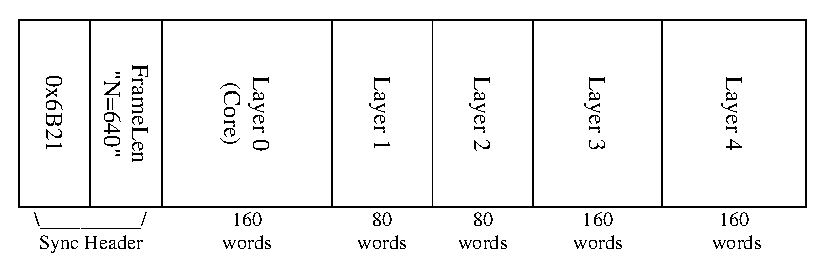
\includegraphics{eidev_fig1ps.eps}
	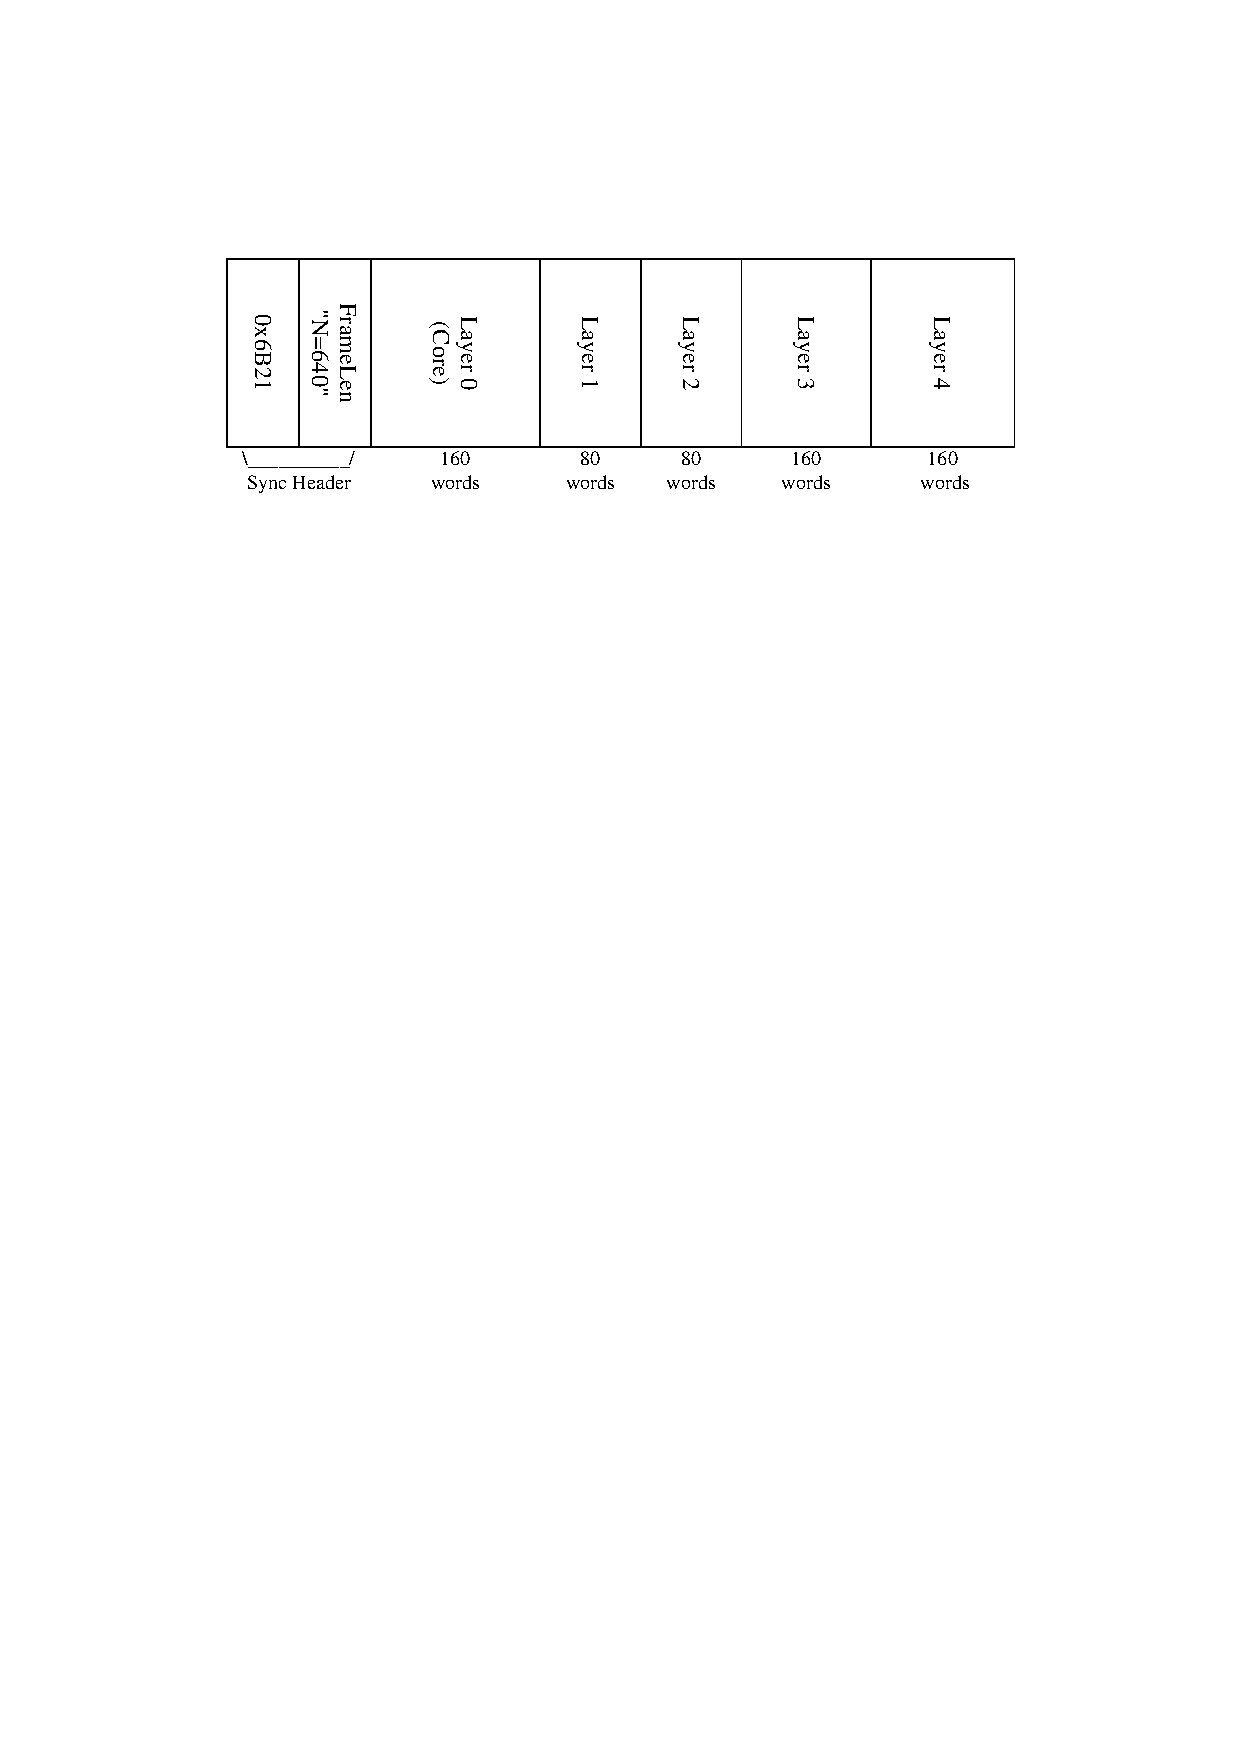
\includegraphics{eidev_fig1}
	\caption{Example G.192 input frame with layering  "-layers 160,240,320,480,640".
	This frame has a size of 640 bits and a G192\_SYNC(0x6B21) header tag.}
	\label{fig:ExampleG192InputFrame}
  \end{center}
\end{figure}

\begin{figure}[htp]
  \begin{center}
%	
\includegraphics{eidev_fig2ps.eps}
	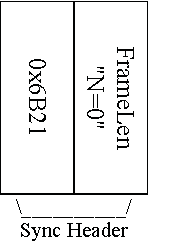
\includegraphics{eidev_fig2}
	\caption{Example G.192 NoData frame, sync tag is G192\_SYNC and frame length 
is zero. NoData frames may be used to simulate DTX (Discontinuous Transmission)
operation.}
	\label{fig:ExampleG192NoDataFrame}
  \end{center}
\end{figure}

%.................................
\newpage
\subsubsection{EID-EV G.192 Output frame examples }
Figure~\ref{fig:G192outputFrameLayer3Error} gives an output frame
example where layer 3 is hit by a layer error in the layered
application mode. Since layer 3 is a lower layer to layer 4 and 5,
those two layers are also truncated from the frame data. In
figure~\ref{fig:G192outputFrameLayer134Error}, the layer 1, 3 and 4
are hit by layer errors in layered error application mode. Here, all
layers above 0 are truncated because layer 1 is
hit. Figure~\ref{fig:G192outputFrameLayer034Error} is an example where
layer 0, 3 and 4 are hit in layered error application mode. All the
layers were deleted because of hit of layer 0, and this is equivalent
to a totally erased frame.

In individual error application modes, the hit layers are filled with
``0''s. In an example give in
figure~\ref{fig:G192outputFrameLayer3ErrorIndividual}, where layer 3
is hit, all he bits in layer 3 are changed to ``0'', and the sync
header is changed to G192\_FER ({\tt 0x6B20}) to indicate the presence
of remaining layers with
errors. Figure~\ref{fig:G192outputFrameLayer134ErrorIndividual} shows
an example where layers 1, 3 and 4 are hit in individual error
application mode, and layer 3 and 4 are truncated with layer 1 filled
with ``0''s. Note here that the Sync header is also changed to
G192\_FER. Finally, for the case where layers 0, 3 and 4 are hit by
layer errors in the individual error application mode, 
figure~\ref{fig:G192outputFrameLayer034ErrorIndividual} gives the
resulting frame. Here, all layers are truncated because layer 0 is
hit.

\begin{figure}[htp]
  \begin{center}
%	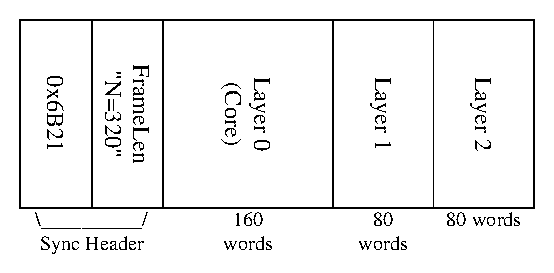
\includegraphics{eidev_fig3ps.eps}
	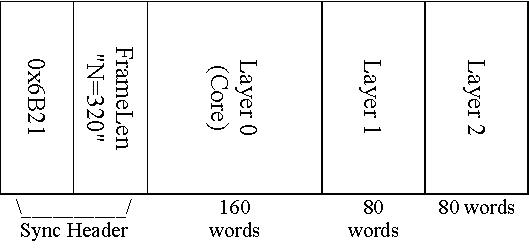
\includegraphics{eidev_fig3}
	\caption{Example G.192 output frame when layer 3 is hit by a layer error 
in the layered error application mode.}
	\label{fig:G192outputFrameLayer3Error}
  \end{center}
\end{figure}

\begin{figure}[htp]
  \begin{center}
%	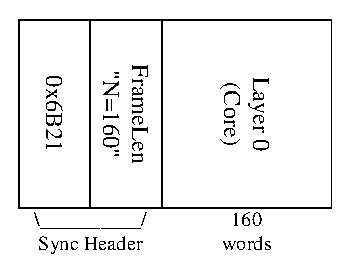
\includegraphics{eidev_fig4ps.eps}
	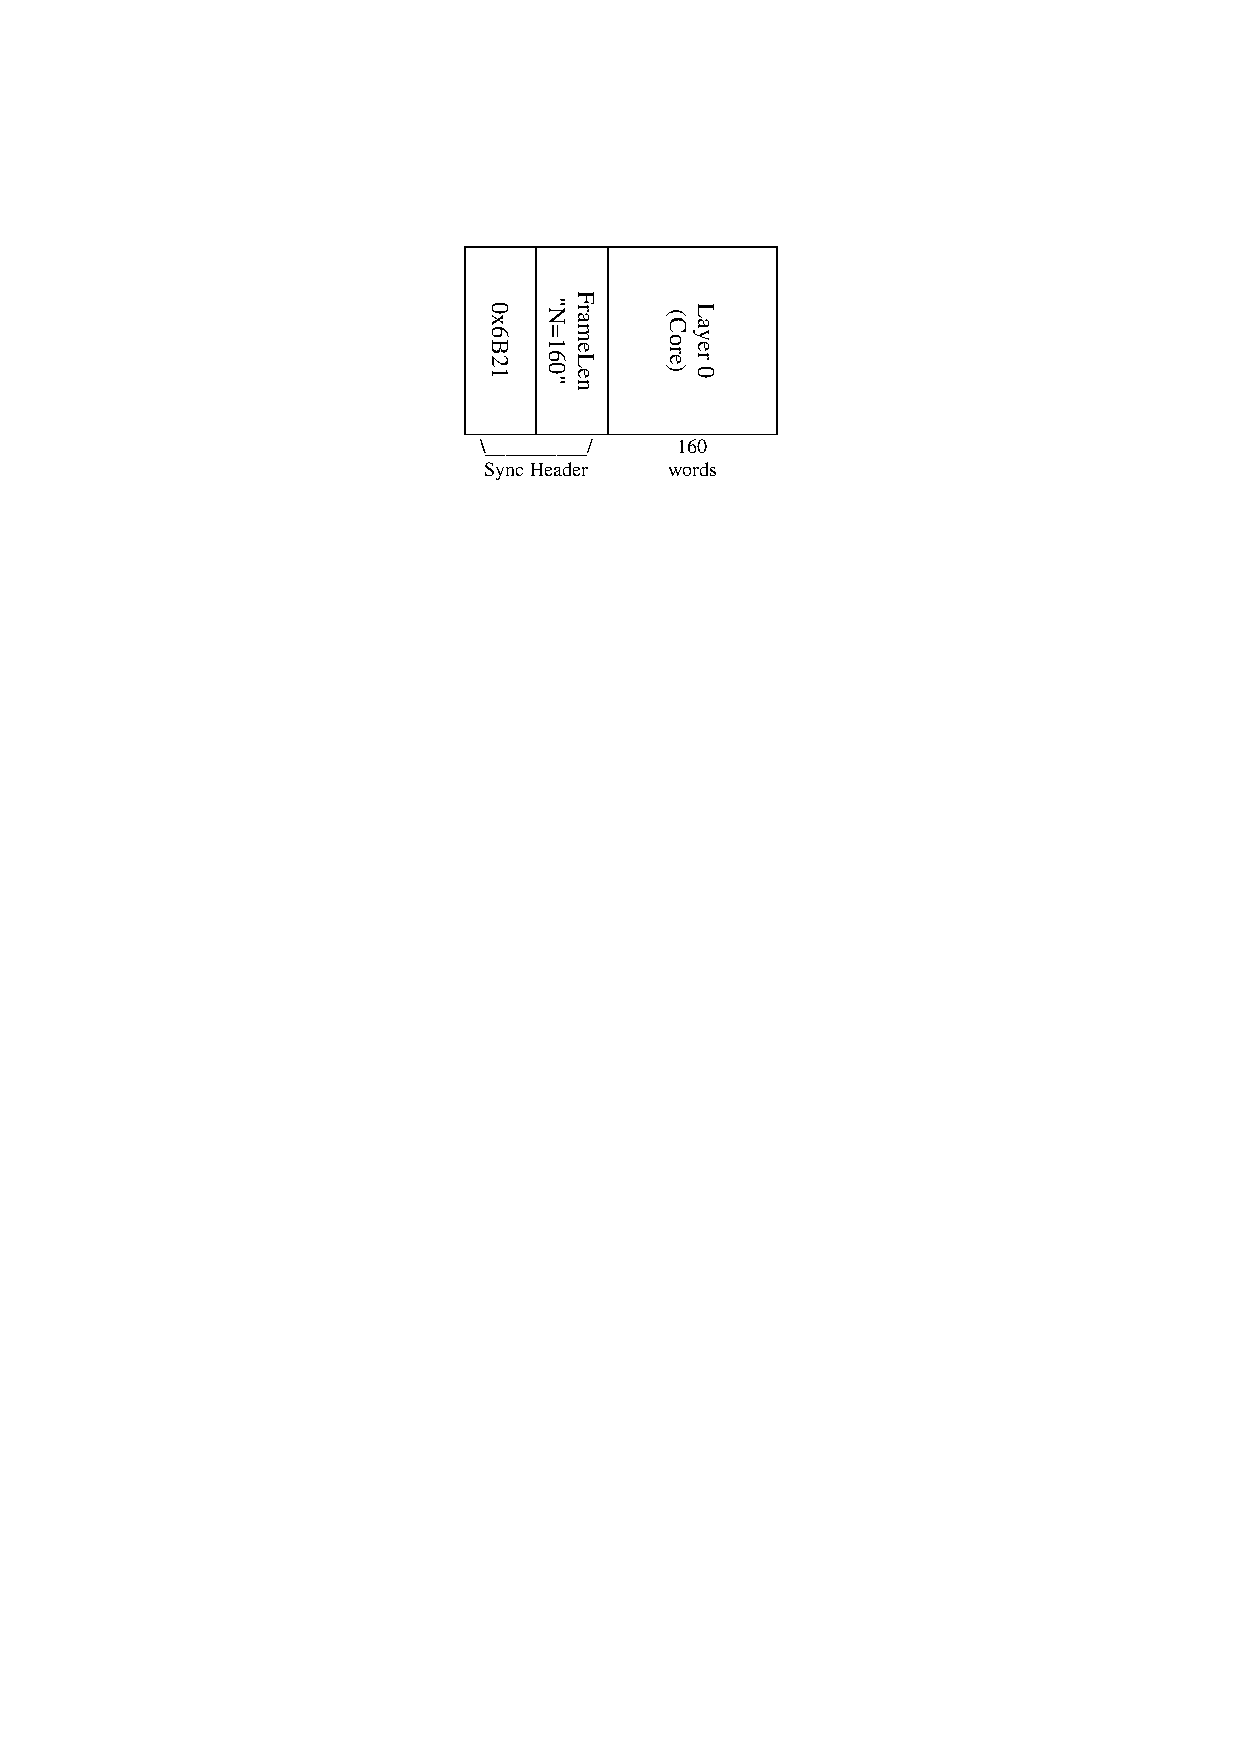
\includegraphics{eidev_fig4}
	\caption{Example G.192 output frame when layer 1, layer 3 and layer 4 
are hit by layer errors in the layered error application mode.}
	\label{fig:G192outputFrameLayer134Error}
  \end{center}
\end{figure}

\begin{figure}[htp]
  \begin{center}
%	
\includegraphics{eidev_fig5ps.eps}
	
\includegraphics{eidev_fig5}
	\caption{Example G.192 output frame when layers 0, 3 and 4 
are hit by layer errors in the layered error application mode.}
	\label{fig:G192outputFrameLayer034Error}
  \end{center}
\end{figure}

\begin{figure}[htp]
  \begin{center}
%	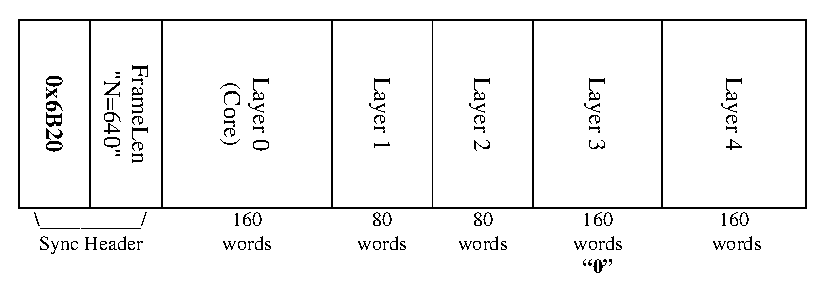
\includegraphics{eidev_fig6ps.eps}
	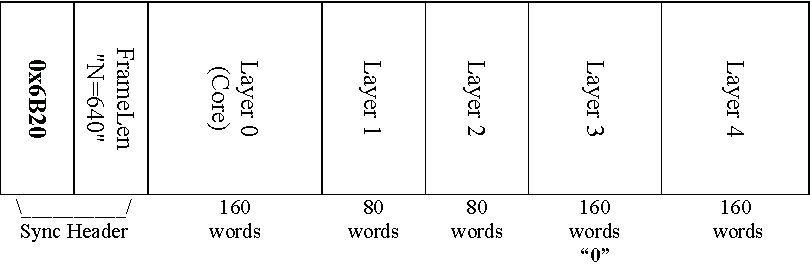
\includegraphics{eidev_fig6}
	\caption{Example G.192 output frame when layer 3 is hit by layer 
errors in the individual error application mode. Note that the Sync 
header is changed to G192\_FER(0x6B20) to indicate the presence of 
remaining layers with errors.}
	\label{fig:G192outputFrameLayer3ErrorIndividual}
  \end{center}
\end{figure}

\begin{figure}[htp]
  \begin{center}
%	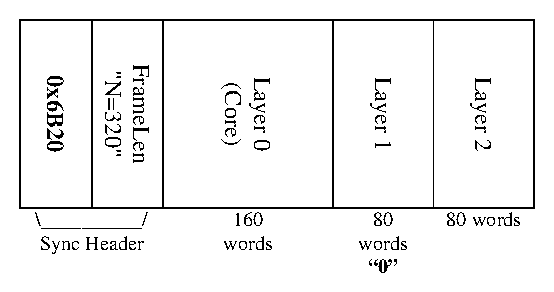
\includegraphics{eidev_fig7ps.eps}
	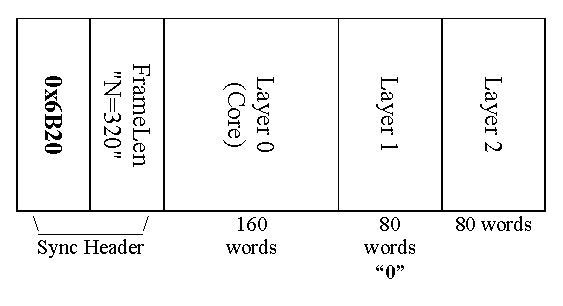
\includegraphics{eidev_fig7}
	\caption{Example G.192 output frame when layers 1, 3 and 4 are hit 
by layer errors in the individual error application mode. Note that 
the frame is truncated and that the Sync header is changed to 
G192\_FER(0x6B20) to indicate the presence of layers with remaining 
errors.}
	\label{fig:G192outputFrameLayer134ErrorIndividual}
  \end{center}
\end{figure}

\begin{figure}[htp]
  \begin{center}
%	
\includegraphics{eidev_fig8ps.eps}
	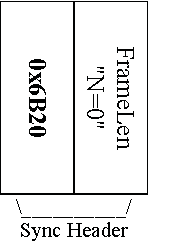
\includegraphics{eidev_fig8}
	\caption{Example G.192 output frame when layers 0, 3 and 4 
are hit by layer errors in the individual error application mode.}
	\label{fig:G192outputFrameLayer034ErrorIndividual}
  \end{center}
\end{figure}
